%Esta charla puede ser descargada en https://github.com/n0rman/charlas/blob/master/GobernanzaInternet/GobernanzaInternet.tex
%Autor: Norman GArcía Aguilar norman@risuep.net

\documentclass{beamer}
%\usepackage[latin1]{inputenc}
\usepackage[spanish]{babel}
\usepackage{graphicx}
\usetheme{Warsaw}
\title{Gobernanza de Internet}
\author[n0rman]{Norman Garc\'ia \\ \texttt{norman@debian.org.ni}}
\institute{Debian Nicaragua}
\date{Abril 25, 2015}
\begin{document}

\begin{frame}
	\titlepage
\end{frame}

%\begin{frame}{Contenido}
%	\tableofcontents
%\end{frame}


\section{Introducci\'on}

\begin{frame}
\frametitle{¿Qu\'e es la Internet?}
	\begin{center}
		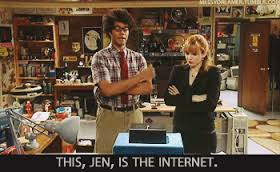
\includegraphics{../img/the-internet.jpeg}
	\end{center}
\end{frame}

\begin{frame}
\frametitle{C\'omo est\'a formada la Internet?}
	\pause Se han definido tres capas que forman la Internet
		\begin{enumerate}
			\pause \item \alert{Infraestructura}: cables, servidores, enrutadores, commutadores.
			\pause \item \alert{Protocolos de comunicac\'on}: reglas, normas que se deben de seguir.
			\pause \item \alert{Informaci\'on}: datos (texto, audio, video).
		\end{enumerate}
\end{frame}

\begin{frame}
	\begin{center}
	            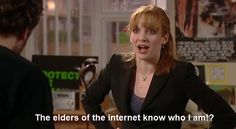
\includegraphics[scale=0.90]{../img/the-elders-of-internet.jpg}
	\end{center}	
\end{frame}

\begin{frame}
\frametitle{Jon postel}
	\begin{itemize}	
		\pause \item Primer miembro de la Internet Society.
		\pause \item Editor \'unico de las \alert{RFC} desde 1969 hasta 1998
		\pause \item Coordinador de \alert{I}nternet \alert{A}ssigned \alert{N}umbers \alert{A}uthority.
		\pause \item \'El junto a una comunidad tomaban las decisiones sobre Internet.
		\pause \item Fue uno de los que redactaron las bases para las reglas de Internet que conocemos hoy en d\'ia.
		\pause \item Uno de los fundadores de Internet y actu\'o como BDFL durante mucho tiempo hasta 1998 cuando muri\'o.
	\end{itemize}
\end{frame}

\begin{frame}
	\begin{center}
	            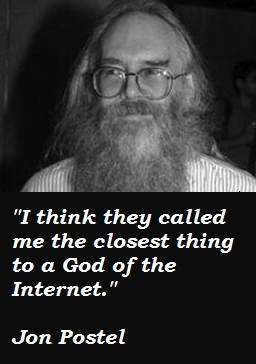
\includegraphics[scale=0.90]{../img/jon-postel.jpg}
	\end{center}	
\end{frame}

\section{Gobernanza}

\begin{frame}
\frametitle{ICANN - IANA}
	\begin{itemize}
		\item \pause IANA hoy en d\'ia es parte del departamento de comercio de U.S.A.
		\item \pause \alert{I}nternet \alert{C}orporation for \alert{A}ssigned \alert{N}ames and \alert{N}umbers, es una organizaci\'on sin fines de lucro creada en 1998 con base en California, USA.
		\item \pause ICANN es la entidad que opera IANA.
		\item \pause Al tener U.S.A juridiscci\'on, puede influir sobre ICANN.
		\item \pause Esto se trata de evitar a trav\'es del modelo Multistakeholder.
	\end{itemize}
\end{frame}

\begin{frame}
\frametitle{Modelo Multistakeholder}
	\begin{center}
		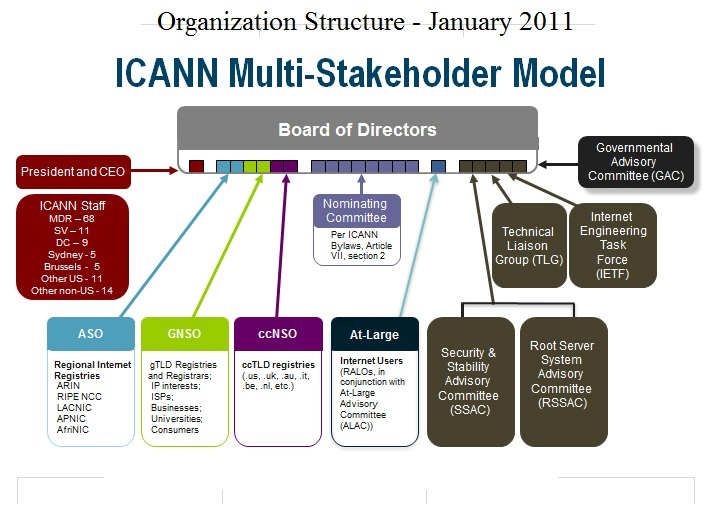
\includegraphics[scale=0.50]{../img/Icann-Organization-Structure-January-2011.jpg}
	\end{center}

\end{frame}

\begin{frame}
\frametitle{Gobernanza de la Internet}
	\begin{itemize}
		\item \pause El desarrollo y aplicaci\'on por Gobiernos, el sector privado y la sociedad civil, en sus respectivos roles, de principios compartidos, normas, reglas, procesos de toma de decisi\'on y programas, que modelan la evoluci\'on y el uso de Internet.
		\item \pause Modelo descentralizado.
		\item \pause Asuntos relacionados con el desarrollo y la aplicaci\'onn de principios, normas, reglas, procedimientos y programas que dan forma a la evoluci\'on y uso de Internet.
     \end{itemize} 
\end{frame}

\section{Gracias}
\begin{frame}
\frametitle{FIN}
	\begin{enumerate}
		\item Presentaci\'on: Gobernanza de Internet
		\item Presentado por: Norman Garc\'ia  \texttt{norman@debian.org.ni}
		\item Abril 25, 2015
		\item Licencia: Creative Commons Atribuci\'on-CompartirIgual 3.0 Unported (CC BY-SA 3.0)
		\item Esta charla puede ser descargada en \texttt{https://github.com/n0rman/charlas}
	\end{enumerate}

	\begin{center}
  		 
\includegraphics[scale=0.20]{../img/cclogo.png}
	\end{center}

\end{frame}
\end{document}
